\newpage
\hypertarget{sec:conBran}{}
\section{Conditional Branching}

\footnotetext{\bf See page xvii of the old handbook for original. This is all new.}

When working with SDMs, you'll often find yourself needing to decide which statement(s) to execute based on the return value of an arbitrary (black box)
operation. In our example so far, we have implemented these constructs via SDM \emph{pattern matching}. 

With eMoflon however, there is an alternate way to
construct these black boxes. In fact, this feature is yet another way of integrating handwritten java code with your SDM! The only ``rule'' of this feature is that your
method must return \texttt{EBoolean}, \texttt{Success}, or \texttt{Failure}, respectively corresponding to \texttt{true} and \texttt{false}. Any other values
will set \texttt{Failure} to \texttt{null}. It follows that void methods cannot be used for branching - an exception will be thrown during execution.


\fancyfoot[R]{ $\triangleright$ \hyperlink{conBran vis}{Next [visual]\hspace{0.2cm} } \\ $\triangleright$ \hyperlink{conBran tex}{Next [textual]} } 

\clearpage
\hypertarget{conBran vis}{}
\subsection{Branching with statement nodes}
\visHeader

\begin{itemize}
  
\item[$\blacktriangleright$] Edit the \texttt{Box} class in your metamodel by invoking the \texttt{Operations} dialogue and create a new method called
\texttt{initalizeBox}. Recalling the sole condition of conditional branching, set its return type to \texttt{EBoolean}. Save the method, then re-open the
\texttt{grow} SDM.

\vspace{0.5cm}

\item[$\blacktriangleright$] Add a new \texttt{StatementNode} from \texttt{addNewPartitionBox} and name it \texttt{initialize}. The edge guard should
automatically set itself to \texttt{failure}.

\vspace{0.5cm}

\item[$\blacktriangleright$] In the \texttt{Statement} tab, invoke a \texttt{MethodCallExpression} to your new method.

\vspace{0.5cm}

\item[$\blacktriangleright$] Finally, attach two \texttt{StopNode}s -- \texttt{true} and \texttt{false} -- along with their appropriate edge guards. These mean
that the if method call succeeds, the box could be initialized, so it will return a literal \texttt{true}. If it failed however, \texttt{box} was already in an
invalid state (by, i.e., having only one card) and returns \texttt{false}. Overall, the new additions to \texttt{box.grow()} should resemble
Fig.~\ref{fig:newGrowControl}.

\vspace{0.5cm}

\begin{figure}[htp]
\begin{center}
  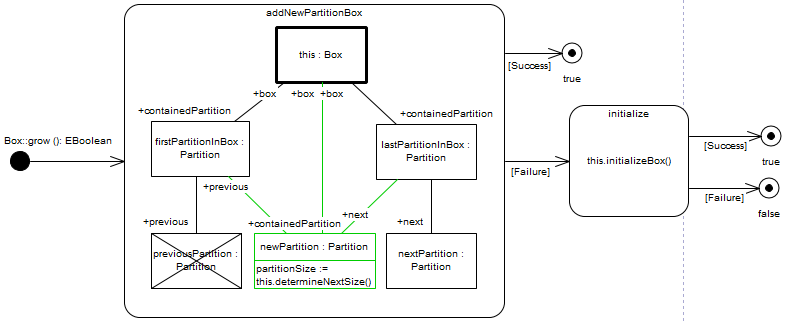
\includegraphics[width=\textwidth]{ea_growAdditions}
  \caption{Extending \texttt{grow} with a \emph{MethodCallExpression}}
  \label{fig:newGrowControl}
\end{center}
\end{figure}

\clearpage

\item[$\blacktriangleright$] Switch back to your open \texttt{Box.grow} SDM in EA. You'll notice that if you double-click on \texttt{initialize}, the
\texttt{Extract Story Pattern} option is invalid. This makes sense -- you don't define a pattern in a statement node. Instead, return to the main diagram and
create a new SDM for \texttt{initializeBox}.

\item[$\blacktriangleright$] In its diagram, create an \texttt{activity node} named \texttt{buildPartitions}. Within it, have a bound \texttt{Box} linked to a
\texttt{onePartition} NAC, and two other `green' (create) object variables, \texttt{firstPartition} and \texttt{lastPartition}. Be sure to also connect two
true/false \texttt{StopNode}s. The pattern should now resemble Fig.~\ref{fig:buildPartitions}. The NAC here can only fulfilled if the box has no partitions,
i.e., is in a pristine state and able to be initialized. In other words, If \texttt{grow} is used for an empty box, it initializes the box for the first time
and grows it after that, ensuring that the box is always in a valid state.

\vspace{0.5cm}
 
\begin{figure}[htp]
\begin{center}
  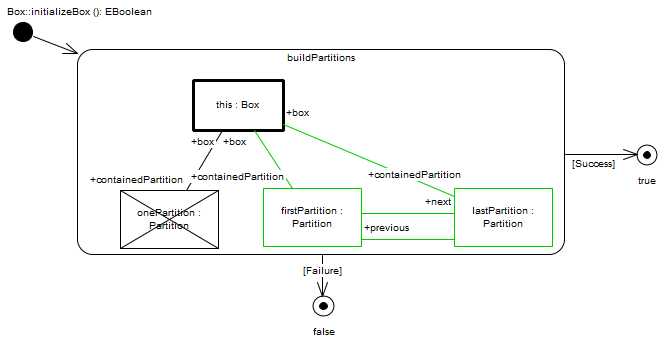
\includegraphics[width=\textwidth]{eclipse_buildPartitions}
  \caption{Compelted NAC to check for \emph{one} partition}
  \label{fig:buildPartitions}
\end{center}
\end{figure}
 
\item[$\blacktriangleright$] You're finished! Save, validate, and build your metamodel, then check out how this is done in the textual syntax in
Fig.~\ref{fig:updateGrow} and Fig.~\ref{fig:pattBuildParts}.

\jumpSingle{initialize notes}

\end{itemize}


\newpage
\hypertarget{conBran tex}{}
\subsection{Branching with statement nodes}
\texHeader

\begin{itemize}

\item[$\blacktriangleright$] Before doing anything else, let's declare the method that will insert two new partitions into \texttt{box} when the original
pattern match fails. Open \texttt{Box.eclass} and add the following signature anywhere in the file: 
\syntax{initializeBox() : EBoolean}

\vspace{0.5cm}

\item[$\blacktriangleright$] Now modify \texttt{Box.grow()} by adding a nested \emph{if/Else} construct, with \texttt{[addNewPartitionBox]} as the
first conditional, and execute a \emph{statement node} if it fails. \texttt{grow} should now resemble Fig.~\ref{fig:updateGrow}.

\vspace{0.5cm}

\begin{figure}[htp]
\begin{center}
  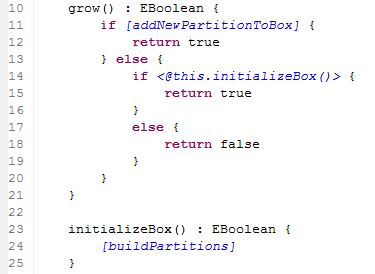
\includegraphics[width=0.5\textwidth]{eclipse_updateGrow}
  \caption{Extending \texttt{Box} with a \emph{statement node}}
  \label{fig:updateGrow}
\end{center}
\end{figure}

\vspace{0.5cm}

\item[$\blacktriangleright$] Next, we want to specify our newest method. Create a new pattern called \texttt{buildPartitions} in its scope. Complete
the pattern as illustrated in Fig.~\ref{fig:pattBuildParts}.

\item[$\blacktriangleright$] As you can see, we have created a NAC that can only be fulfilled if the box has no lonely partition. In turn, this means that if a
box is completely empty, it will be intialized for the first time with two partitions, and guaranteed to remain in a valid state if growing continues.

\clearpage

\vspace*{2cm}

\begin{figure}[htp]
\begin{center}
  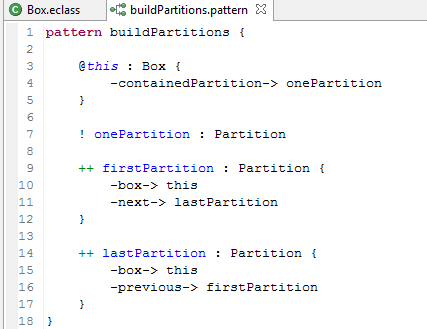
\includegraphics[width=0.7\textwidth]{eclipse_buildPartitionsPattern}
  \caption{NAC initalizing an empty box}
  \label{fig:pattBuildParts}
\end{center}
\end{figure}

\item[$\blacktriangleright$] That's it! Save and build your metamodel to make sure no errors exist. To see how this is depicted in the visual syntax, check out
Fig.~\ref{fig:newGrowControl} and Fig.~\ref{fig:buildPartitions}.

\end{itemize}

